\section{Kaka Kamaludin (1174067)}
\subsection{Buku}
belum bayar
\subsection{Data Geospasial}
\begin{itemize}
Data geospasial (GD) adalah informasi yang entah bagaimana dilampirkan ke lokasi objek tertentu. Biasanya, informasi ini disimpan dalam bentuk koordinat geografis dan topologi. Jumlah data tersebut tumbuh pada tingkat yang mengejutkan, karena sebagian besar dibuat bukan oleh orang-orang, tetapi oleh berbagai perangkat.
	Data geografis berisi empat komponen terintegrasi:
	\item lokasi
	\item properti dan karakteristik
	\item hubungan sosial
	\item waktu
Dengan demikian, dalam GIS, data geospasial direpresentasikan dalam dua kategori yaitu spasial(lokasi) dan non-spasial(atribut). Data spasial dapat mencakup fitur geografis yang diwakili oleh:
 	\item titik, mewakili pohon, tiang lampu, atau beberapa objek yang lokasinya dijelaskan oleh satu titik.
 	\item garis,  adalah objek nyata yang dapat dianggap sebagai garis. Busur terdiri dari segmen garis dan busur lingkaran. Di dunia nyata, busur dapat berupa jalan, sungai, saluran transmisi listrik atau utilitas bawah tanah, misalnya, sistem saluran air dan saluran pembuangan.
 	\item Poligon adalah area tertutup yang mewakili area yang homogen dengan beberapa kriteria. Poligon menunjukkan jenis tanah, konstituensi, plot tanah atau kontur bangunan.
 
Data atribut dapat mencakup pengidentifikasi objek, informasi deskriptif apa pun dari basis data, gambar, dan banyak lagi.
\subsection{Link}
https://youtu.be/vNbo-W3Beio
\subsection{Plagiarism}
\begin{figure}[H]
	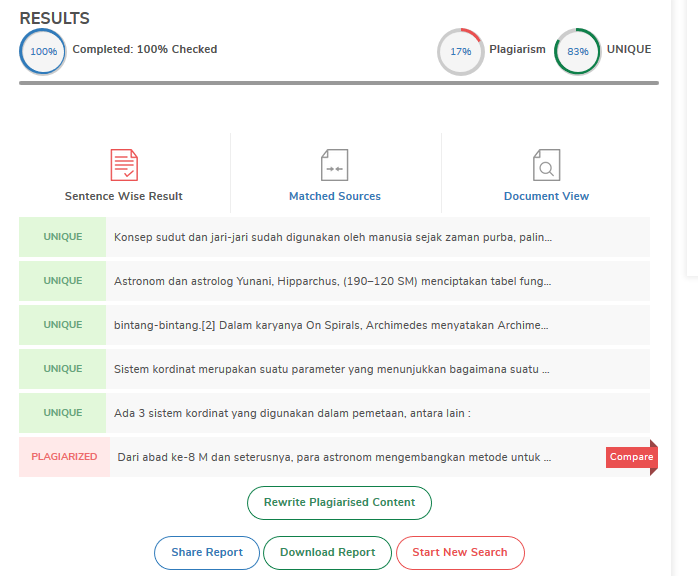
\includegraphics[width=4cm]{figures/Tugas1/1174074/plagiat.png}
	\centering
	\caption{Gambar Plagiat}
\end{figure}
\subsection{Cara Penggunaan}
\subsubsection{Gambar}

\hfill\break

Contoh Gambar
\begin{figure}[H]
	\includegraphics[width=4cm]{figures/himatif.png}
	\centering
	\caption{Contoh gambar.}
\end{figure}

\subsubsection{List}
\begin{enumerate}
	\item Satu
	\item Dua
\end{enumerate}

\begin{itemize}
	\item Satu
	\item Dua
\end{itemize}

\end{document}